% icstdoc.tex V1.12 6 May 2011

\documentclass[fonts]{icst}

\usepackage{moreverb}

\usepackage[breaklinks,colorlinks,bookmarksopen,bookmarksnumbered,linkcolor=ICSTblue,citecolor=blue,urlcolor=ICSTblue]{hyperref}
\def\UrlBreaks{\do\/\do-\do.}

\usepackage{breakurl}
\usepackage{doi}

\usepackage{subcaption}


\newcommand\BibTeX{{\rmfamily B\kern-.05em \textsc{i\kern-.025em b}\kern-.08em
T\kern-.1667em\lower.7ex\hbox{E}\kern-.125emX}}

\def\volumeyear{2019}

\journalname{XXXXXX}
\articletype{Research Article/Editorial}
\setcounter{page}{01}
 \def\volumeyear{XXXX}
 \def\volumenumber{XX}
  \def\issuemonth{XX-XX}
  \def\issuenumber{X}
  \def\articleid{XX}
  \def\copyrightholder{Andrew Meyer\textit{ et al.}, licensed to ICST}
  \copyrightnote{This is an open access article distributed under the terms of the Creative Commons Attribution license (\url{http://creativecommons.org/licenses/by/3.0/}), which permits unlimited use, distribution and reproduction in any medium so long as the original work is properly cited.}
  \def\articledoi{10.4108/XX.X.X.XX}
\received{XXXX}
  \accepted{XXXX}
  \published{XXXX}

\begin{document}

\runningheads{A. Meyer, S. Roy}{NIST Standards Compliance of Metadata-Based Deleted-File-Recovery (DFR) Tools}

\title{NIST Standards Compliance of Metadata-Based Deleted-File-Recovery (DFR) Tools}

\author{Andrew Meyer\affil{1}\fnoteref{1}, Sankardas Roy\affil{2}\fnoteref{2}}

\address{\affilnum{1}Bowling Green State University, Bowling Green, Ohio, USA\\
\affilnum{2}Bowling Green State University, Bowling Green, Ohio, USA}

\abstract{Digital forensics (DF) tools are used for post-mortem investigation of cyber-crimes. 
National Institute of Standards and Technology (NIST) 
has set standards for DF tools. Compliance with the standards by DF tools is critical to ensure 
integrity of the outcome of forensics analysis. 
In this paper, we consider standardization of one class of DF tools which are for Deleted File Recovery (DFR). 
We design an exhaustive list of canonical test file system images to evaluate a DFR tool.
Via extensive experiments we find that many popular DFR tools do not satisfy some of the standards, and 
we compile a comparative analysis of these tools, which could help the user choose the right tool. 
Furthermore, one of our research questions identifies the factors which make a DFR tool fail. 
Moreover, we also provide critique on applicability of the standards. 
Our findings is likely to trigger more research on compliance of standards from the researcher community as well as the practitioners.}

\keywords{Deleted File Recovery, Digital Forensics, Metadata, NIST Standards, File System, FAT, NTFS}

%\tnotetext[1]{Please ensure that you use the most up to date
%class file, available from EAI at \url{http://doc.eai.eu/publications/transactions/latex/}
%}

\fnotetext[1]{Corresponding author.  Email: \email{apmeyer@bgsu.edu}}
\fnotetext[2]{Corresponding author.  Email: \email{sanroy@bgsu.edu}}

\maketitle


\section{Introduction}

Both in corporate and government settings, digital forensic (DF) tools are used for post-mortem investigation of cyber-crimes and cyber-attacks. 
Nowadays it is common \cite{df:news} for the police to use DF tools to follow an eletronic trail of evidence to track down the suspect. 
To maintain the quality and integrity of DF tools, National Institute of Standards and Technology (NIST)'s 
Computer Forensics Tool Testing Program (CFTT) \cite{cftt:nist} 
set standards for these tools. Maintaining the standards of DF tools 
is especially critical for judicial proceedings: usage of a forensic tool that does not follow the standards may cause evidence to be thrown 
out in a court case whereas incorrect results from a forensic tool can also lead improper prosecution of an innocent defendant. 

The focus of this paper is about standardization of one class of DF 
tools that are for Deleted File Recovery (DFR) \cite{meta:dfr:standards}. 
As the name suggests, a DFR tool attempts to retrieve deleted files
from a file system of a computer. As an example, given a hard disk or a USB drive 
(which might have been seized from the suspect computer or collected from the crime scene), a 
forensics professional can use a DFR tool to investigate about (and potentially retrieve) deleted files that 
a suspect may have deleted to hide important information. 
The success or failure of a DFR tool can decide the outcome of a case.  

DFR tools are typically classified as one of two varieties, corresponding to two different approaches to file recovery.
These varieties are \emph{metadata-based} tools and \emph{file carving} tools.
The focus of this paper is metadata-based DFR tools, with file carving left for future work.
In the rest of the paper, unless otherwise mentioned, by \emph{DFR tool} we mean metadata-based DFR tool.

Our experiments with a popular DF tool suite named Autopsy~\cite{autopsy} 
show that it does not satisfy all NIST standards for DFR. 
Furthermore, we extensively experimented with other frequently used DFR tools. 
We compare those tools' performance and compile a comparative analysis, which could help the user choose the right DFR tool. 

Evaluating the performance of a DFR tool is complex because many elements of a forensics scenario determine 
the success or failure of the file recovery process. 
A few such factors are the type of the file system (FAT, NTFS, etc.), presence of other active/deleted 
files in the file system, fragmentation of a file, a deleted file being overwritten by another file, and so on.
So, comparison of two DFR tools is scientific only if they are compared while keeping these factors same. 
Via extensive analysis, we design a set of test file system images (for either of FAT and NTFS) which considers each of the above factors independently. 
We claim that this list of test cases is exhaustive and thus claim that our evaluation gives a complete picture. 

As there are many file systems (e.g., ext4, HFS, etc.) in addition to FAT and NTFS, one might be interested to know why we chose FAT and NTFS for the current work. 
Because FAT and NTFS are very widely used on external storage devices and devices running Microsoft Windows, respectively,
real-life forensics investigation often involves these two file systems.
While we leave other file systems for future study, our current methodology could be 
used on other file systems to make a similar study.

The main contributions of the paper are listed as follows:
\begin{itemize}
\item We design and build an exhaustive list of canonical test file system (FAT and NTFS) images to test the DFR tool per NIST standards. 
\item We perform evaluation of frequently-used DFR tools (including free tools as well as proprietary ones) on the test images.
\item For the interesting cases of tools' success or failure, we provide logical explanation.
\item We provide critique on applicability of some of the NIST standards in a practical setting. 
\end{itemize}


The NIST CFTT portal currently publishes reports of only a subset of DFR tools. 
However, the scope of tools needs to be expanded as many new tools come to market and become popular.
Also, existing DFR tools should be retested to ensure their reliability is consistent 
as new patches and features come out. 
Adding new reports to the CFTT website will allow tool developers a 
chance to continually develop their tool for the better. We will submit our study reports to the CFTT portal.

As a side benefit, our work leads to a few hands-on lab-modules to be used in digital forensics courses 
at BGSU, enriching the new DF specialization program in the CS department. We will also make these modules
available for relevant instructors at other universities.

\section{Research Questions} \label{rqs}

DFR tools, which come in both metadata-based and file carving variants, are software for recovering deleted data from a digital storage device.
We evaluate a selection of DFR tools according to guidelines set by NIST CFTT.
We specifically investigate the following research questions (RQs):

\begin{itemize}
\item[RQ1.] How well do our selected metadata-based DFR tools meet each of the NIST CFTT guidelines?

\item[RQ2.] What conditions influence the success and failure of metadata-based DFR tools?

\item[RQ3.] How well do our selected file carving tools meet each of the NIST CFTT guidelines?

\item[RQ4.] What conditions influence the success and failure of file carving tools?
\end{itemize}


 

\section{Background}

\begin{paraphrase}
 In this section, we present some of design basics (often simplified to aid readability) of FAT file system and NTFS file system, 
which are relevant to what we discuss in the latter part of the paper. 
We highlight what information remains in the file system after a file is deleted, 
which leads to understanding of how metadata-based file-recovery might work. 
Finally, we present the \emph{core features} of NIST standards for such recovery tools.  
\end{paraphrase}

\TODO{Add a few lines about carving}


\subsection{FAT File System}
\begin{paraphrase}
 As in many other file systems, a file in FAT system has metadata in addition to the actual file content. 
The main metadata of a file (say foo.txt) in FAT system is called a \emph{directory entry}, which is of 32 bytes.
The directory entry of a file (say foo.txt) has three main \emph{essential} elements: (a) file name, (b) file size, and 
(c) index of the starting cluster (which holds the actual file content). We can figure 
out the index of other clusters of the file by reading a global table called the FAT table. The FAT table
can determine the chain of clusters which hold the data of a file. In particular, 
for each cluster (say x) of the file system, the FAT table has an entry, and 
if FAT(x) is 0, then that means cluster x is currently unallocated. 
On the other hand, if FAT(x) is y, then that means cluster y is the next cluster after cluster x (as part of the same file).
If FAT(x) is EOF, that indicates cluster x is the last cluster of the file.
   
As an example, the directory entry of foo.txt and the clusters (holding the actual content of foo.txt) 
are illustrated in Figure~\ref{fig:fat1}. The FAT table is also shown, which tells us that foo.txt's data is stored 
in contiguous clusters, starting from cluster 100 and ending at cluster 200.

% \begin{figure}[h]
%     \centering
%     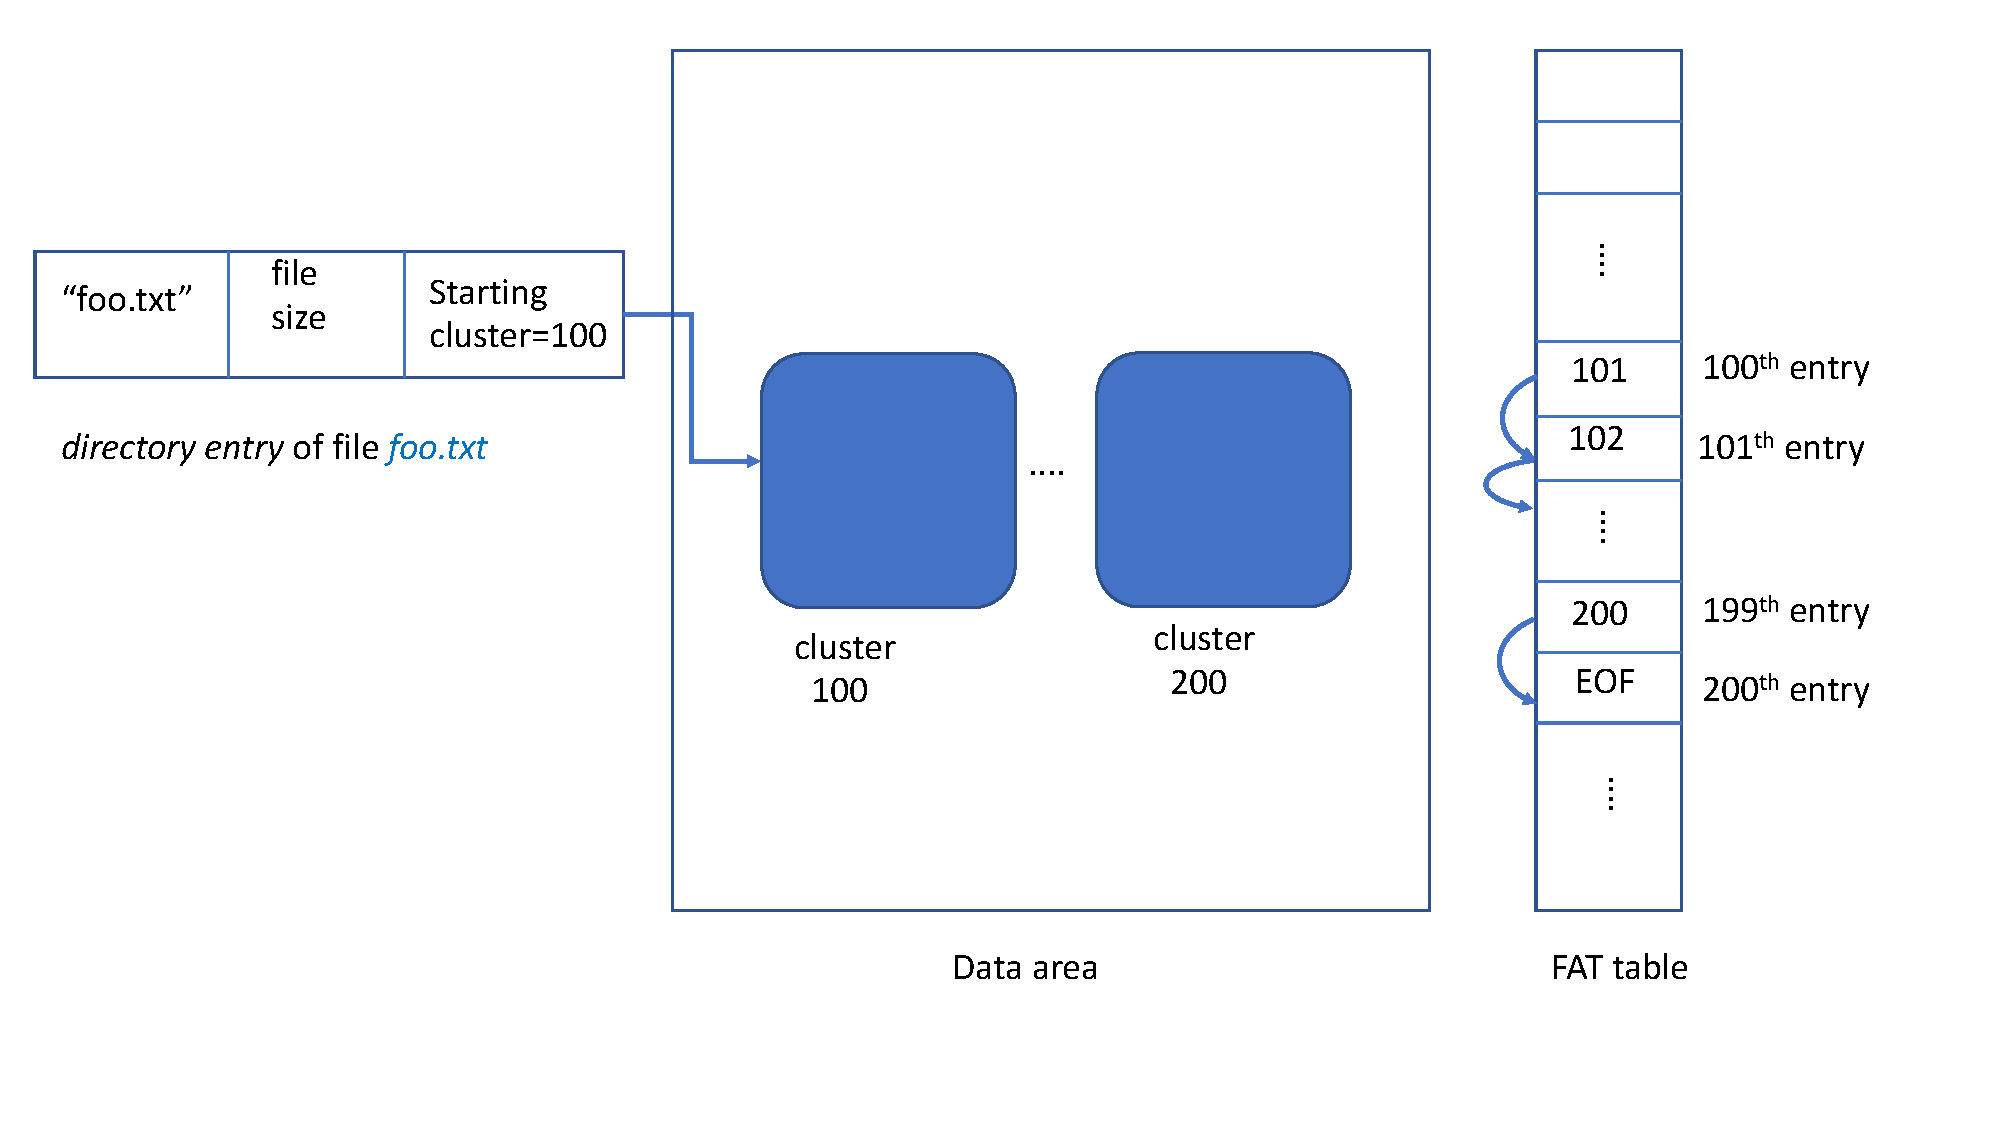
\includegraphics[width=\linewidth]{fig/fat1.pdf}
%     \caption{File foo.txt in a FAT file system. The \emph{directory entry} of this file and the actual file content clusters (shaded) are shown. 
% The FAT table is also shown, which determines the chain of clusters (from cluster 100 to cluster 200) of foo.txt.}
%     \label{fig:fat1}
% \end{figure}


The change in metadata and actual content of foo.txt is illustrated in Figure~\ref{fig:fat2} after the file is deleted.
The first character of the file name (say ``foo.txt") is flagged (``\_oo.txt") to denote that the file is deleted, 
but the remaining part of the directory entry can be still available. In the FAT table, the deleted file's corresponding
entries are \emph{zeroed}, which denotes that those clusters are available to be allocated to a new file (if necessary).
However, the actual content carrying clusters (say cluster 100 to cluster 200)
can still be intact until they are \emph{overwritten} by another file. 
  
% \begin{figure}[h]
%     \centering
%     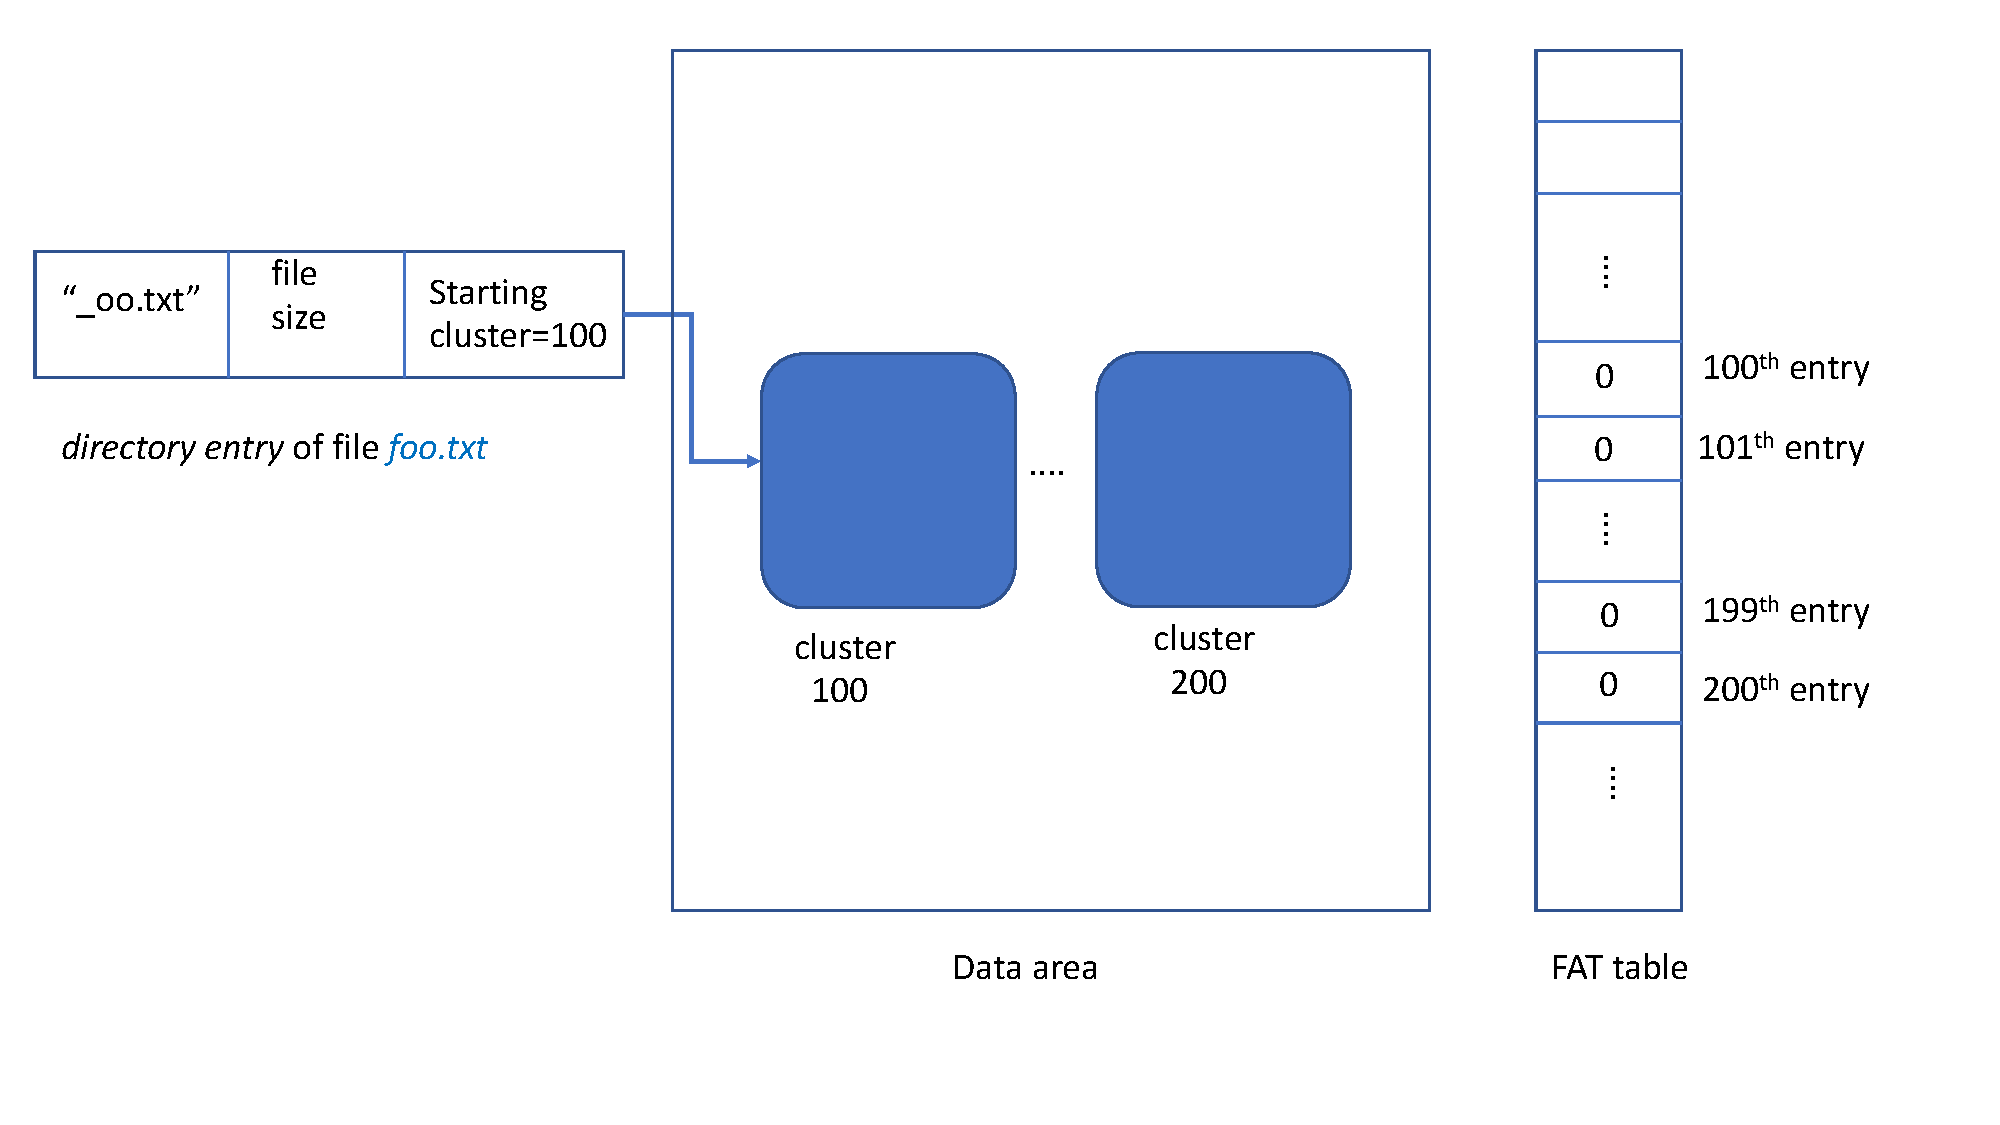
\includegraphics[width=\linewidth]{fig/fat2.pdf}
%     \caption{The metadata and actual content of foo.txt are shown after the file is deleted whereas the corresponding entries (i.e., 100-200) in the FAT table are zeroed.}
%     \label{fig:fat2}
% \end{figure}

Furthermore, it is possible that the content of a file is not stored in contiguous clusters in FAT file system, 
and this phenomenon is called \emph{fragmentation}.
If the original file foo.txt has two fragments, it may look as illustrated in Figure~\ref{fig:fat3} where the file's first fragment is from cluster 100 to cluster 101 and the 
second fragment is from cluster 200 to cluster 298. 

% \begin{figure}[h]
%     \centering
%     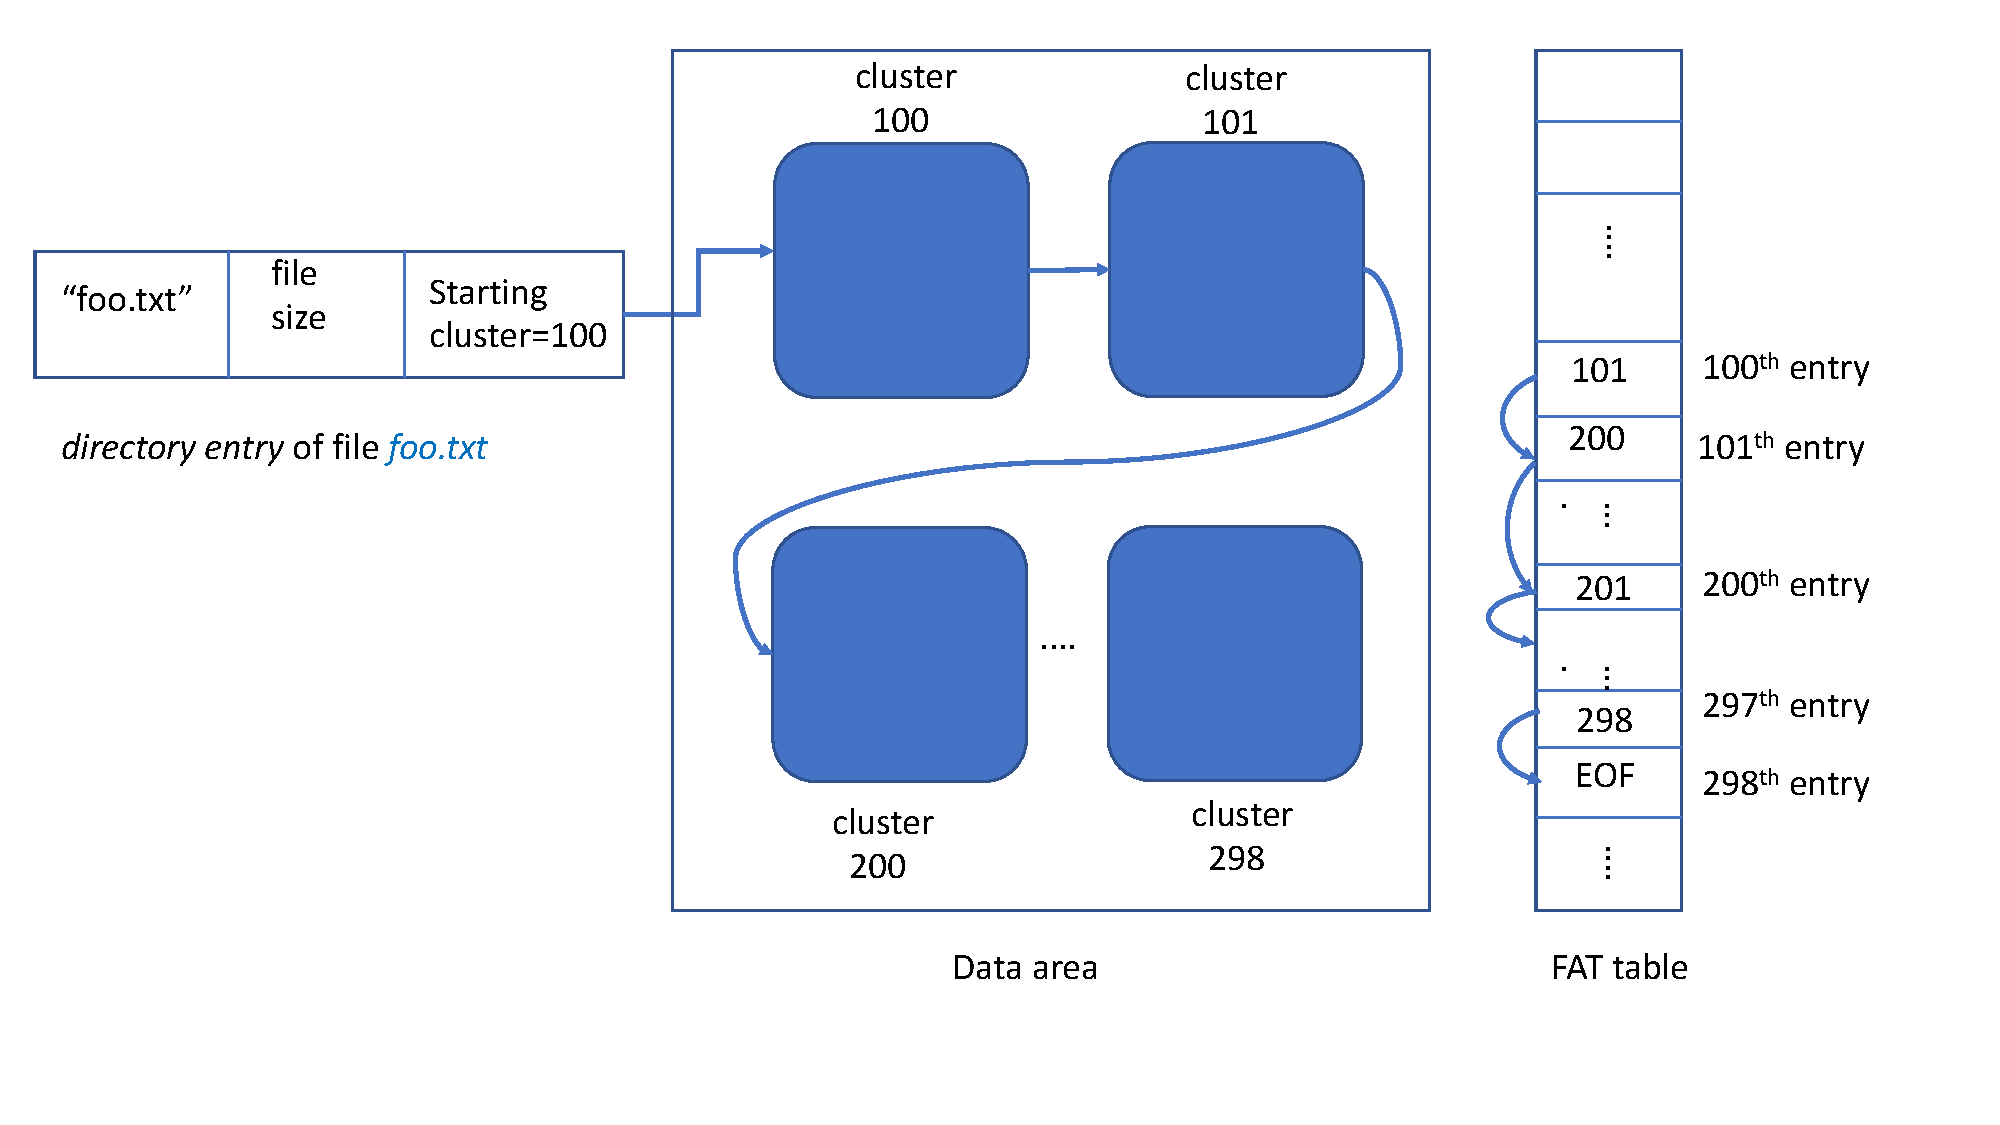
\includegraphics[width=\linewidth]{fig/fat3.pdf}
%     \caption{The layout of metadata and actual content of a file foo.txt is shown whereas the file has two fragments (cluster 100-101 and cluster 200-298) 
% as determined by the FAT table.}
%     \label{fig:fat3}
% \end{figure}
\end{paraphrase}



\subsection{NTFS File System}
\begin{paraphrase}

In an NTFS system, each file has an entry in the Master File Table (MFT) where every entry is typically 1024 bytes. 
If a file is short, then all of its metadata as well as the actual content can sit inside the MFT entry; otherwise, 
the file content can be non-resident (i.e., not in MFT entry) and located in other clusters.
  
As an example, the MFT entry of foo.txt and the actual content carrying clusters are illustrated in Figure~\ref{fig:ntfs}.
The MFT entry indicates that there are two runs of clusters (100-101 and 200-298) which carry the actual file content. 
In this case, the example file has two fragments.

% \begin{figure}[h]
%     \centering
%     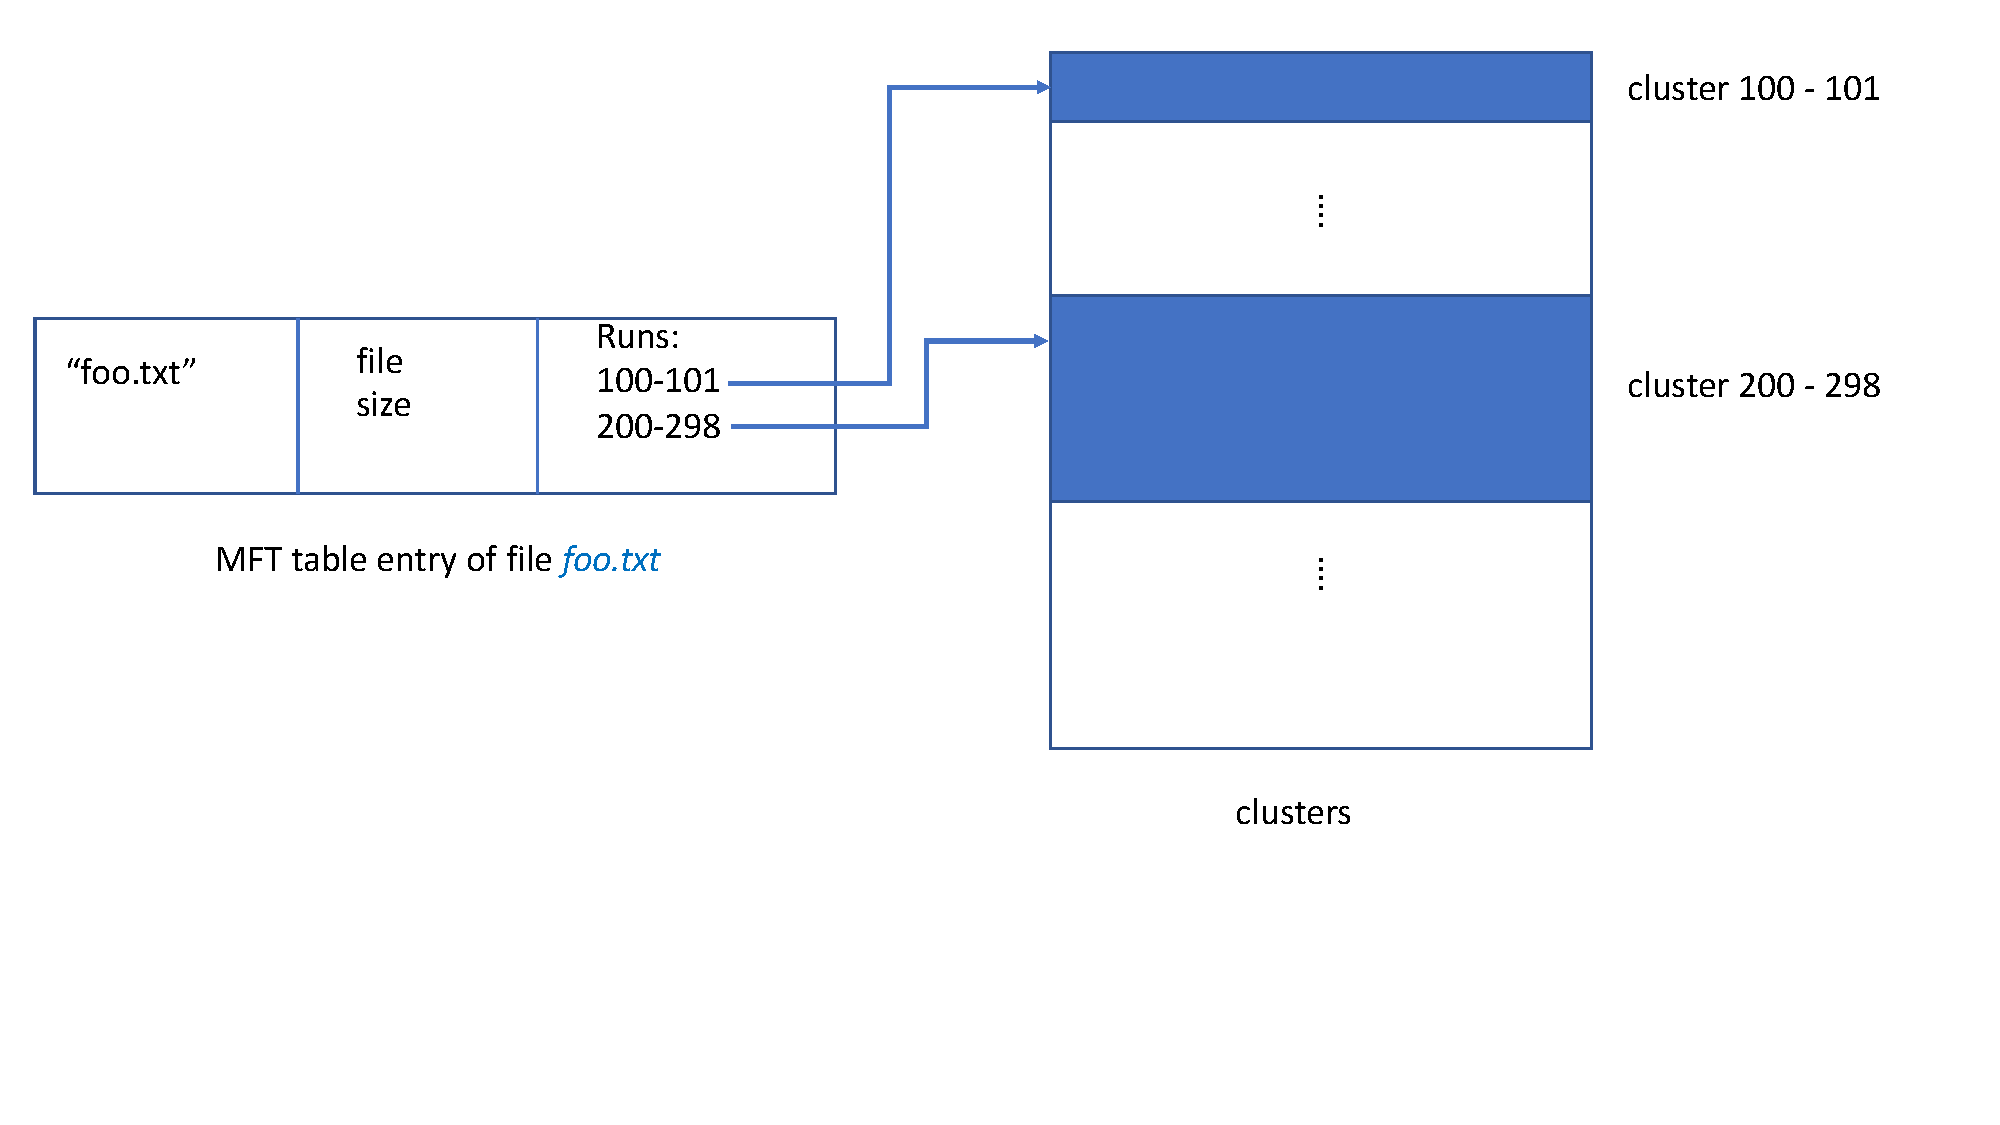
\includegraphics[width=\linewidth]{fig/ntfs.pdf}
%     \caption{To illustrate NTFS file system, the MFT entry of foo.txt and the actual content carrying clusters are shown. 
% This file has two fragments (cluster 100-101 and cluster 200-298).}
%     \label{fig:ntfs}
% \end{figure}
 
\end{paraphrase}

\subsection{Metadata-Based Deleted File Recovery}
\begin{paraphrase}
 The previous discussion implies that in many cases a deleted file's metadata 
(e.g., directory entry in FAT or MFT entry in NTFS) can be still available, 
and it is possible to recover the file content using this metadata. 
This is called metadata-based deleted file recovery.

For instance, in the example of Figure~\ref{fig:fat2},
we can see from the directory entry of foo.txt that 
the deleted file starts in cluster 100 and has a size of 101 clusters;
thus, we can reason that the deleted file content is in cluster 100 to cluster 200.
We can recover the whole file via reading the raw content of these clusters (e.g., by using dd command in Kali Linux). 

Note that in FAT system the \emph{directory entry} of a file only refers to the starting cluster, and it does not carry any information about the file fragments.
That is why in certain situations where the deleted file is fragmented, metadata-based file recovery in FAT system encounters challenges.
On the other hand, if a file is fragmented in NTFS, the corresponding MFT entry does contain information on all the runs (i.e., fragments) of the file
(as shown in Figure~\ref{fig:ntfs}). Consequently, fragmentation does not introduce any extra challenge in file recovery in NTFS.
\end{paraphrase}

\subsection{File Carving}

\TODO{TODO}

\subsection{NIST Guidelines}
\subsubsection{For Metadata-Based DFR}
\begin{paraphrase}
 The NIST guidelines~\cite{meta:dfr:standards} list four \emph{core features} upon which metadata-based DFR tools are to be judged.
Following is the text of each core feature as well as our interpretation of each in the context of this work:
\begin{itemize}
 \item[\textbf{DFR-CR-01}] ``The tool shall identify all deleted File System-Object entries accessible in residual metadata''~\cite{meta:dfr:standards}.
 We consider a tool passing this standard if it identifies to the user each file system metadata entry that is marked as deleted.
 \item[\textbf{DFR-CR-02}] ``The tool shall construct a Recovered Object for each deleted File System-Object entry accessible in residual metadata''~\cite{meta:dfr:standards}.
 We consider a tool passing this standard as long as it outputs a file for each deleted file, even if the output file is empty.
 \item[\textbf{DFR-CR-03}] ``Each Recovered Object shall include all non-allocated data blocks identified in a residual metadata entry''~\cite{meta:dfr:standards}.
 For FAT file systems, we consider a tool passing this standard if it recovers at least the first contiguous segment of unallocated sectors starting 
from the first sector originally allocated to the deleted file. For NTFS file systems, the tool must recover all unallocated sectors originally allocated to the deleted file.
 \item[\textbf{DFR-CR-04}] ``Each Recovered Object shall consist only of data blocks from the Deleted Block Pool''~\cite{meta:dfr:standards}.
 We consider a tool passing this standard if the recovered file consists only of data from the original deleted file, or null data to represent omitted portions.
\end{itemize}

\end{paraphrase}

\subsubsection{For File Carving} \label{sec:carving_features}

\begin{paraphrase}
 The NIST guidelines~\cite{carving_standards} list five \emph{core features} upon which file carving DFR tools are to be judged.
Following is the text of each core feature as well as our interpretation of each in the context of this work:
\end{paraphrase}
\begin{itemize}
 \item[\textbf{FC-CR-01}] ``The tool shall return one carved file for each supported file header signature from a source file that is present in the search arena''.~\cite{carving_standards}
 
 Each file from the original disk will begin with a header signature specific to its file format. We consider a tool as passing this guideline if it carves a file starting at each of those header signatures.
 In other words, tools that perform well on this core feature have a high ``hit rate.''
 
 \item[\textbf{FC-CR-02}] ``A carved file shall only contain data blocks from the search arena''.~\cite{carving_standards}
 
 In other words, the tool should only work within the drive or partition it is given, and should not try to carve from out-of-bounds.
 
 \item[\textbf{FC-CR-03}] ``All data blocks in a carved file shall originate in a single source file''.~\cite{carving_standards}
 
We consider a tool as passing if each recovered file only contains data from one file on the original disk.
 
 \item[\textbf{FC-CR-04}] ``The file type of a carved file shall match the file type of its contents''.~\cite{carving_standards}
 
 We interpret this to mean that the file extension given to a recovered file must accurately describe the format of the file data. We exclude false positives from this evaluation because their data is highly unlikely to be of any file format. So, we only consider files which were carved starting from a valid header signature.
 
 \item[\textbf{FC-CR-05}] ``The tool shall return carved files in a state that conforms to a valid file of the carved file type''.~\cite{carving_standards}
 
 We consider a tool as passing if each recovered file can be parsed without error by some application software.
 We use the ImageMagick tool suide to evaluate this.
\end{itemize}

\section{Approach}

\subsection{Overview}

To test the DFR tools, we first designed hypothetical test scenarios involving factors which would make recovery difficult. We then created each scenario in real filesystems and saved them as raw images. Using the images as input, we ran each DFR tool and attempted to recover all deleted files. Finally, we compared the recovered files to their original versions in order to judge the tools' compliance with the NIST standards.  \ref{fig:overview}

\begin{figure}[h]
    \centering
    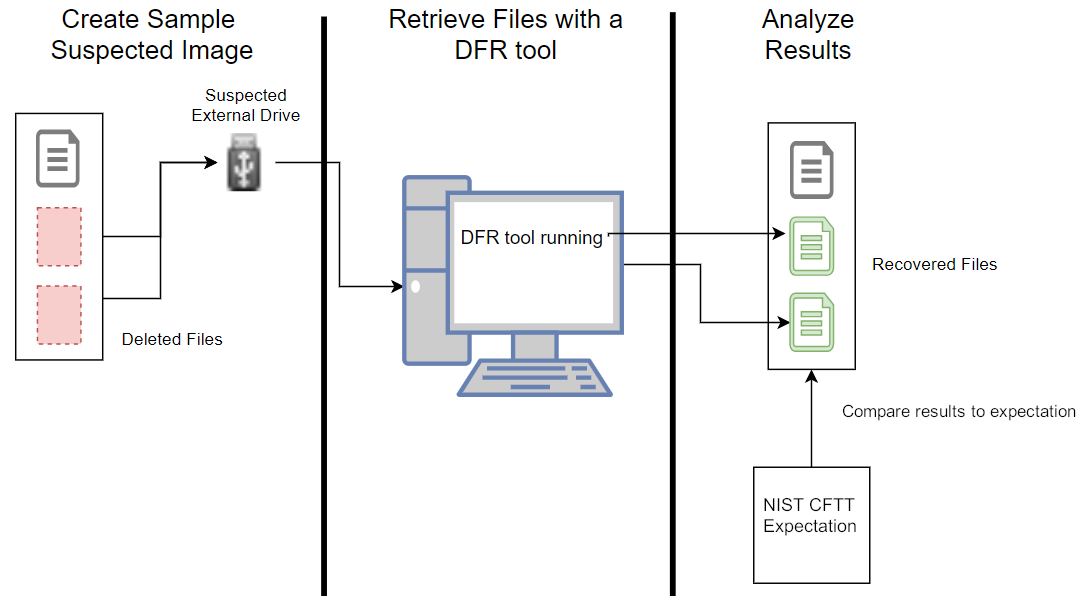
\includegraphics[width=\linewidth]{fig/overview.png}
    \caption{The DFR tool targets to retrieve deleted files. The recovery accuracy is compared to the NIST CFTT standard.}
    \label{fig:overview}
\end{figure}

\subsection{Designing Recovery Scenarios}
To test the DFR tools' compliance with the standards, we designed a variety of scenarios in which a tool might have to recover a deleted file. We started with the simplest possible case: a filesystem containing just one deleted file. This case is ideal and trivial, but by adding more files, we can create far more complex scenarios.

% Fragmentation and Overwriting are the two things that can complicate file recovery 
The NIST standards limit the scope of testing to situations in which files were ``created and deleted in a process similar to how an end-user would create and delete files,''\cite{meta:dfr:standards} and  exclude ``files and file system metadata that is specifically corrupted, modified, or otherwise manipulated to appear deleted.''\cite{meta:dfr:standards}
Within these constraints, there are two factors which can significantly complicate the file recovery process: fragmentation, and overwriting. \comment{need to make sure these are defined elsewhere, if not they should be defined here}

% Make different varieties of Fragmentation and overwriting, and combinations
These factors are thus the focus of our test scenarios, with all cases besides the first involving either fragmented files, overwritten files, or a combination of both.

We designed the following test cases:
\begin{itemize}
    \item [1] Single deleted file
    \item [2] Deleted file fragmented around an active file\ref{fig:case_2}
    \begin{figure}[h]
        \centering
        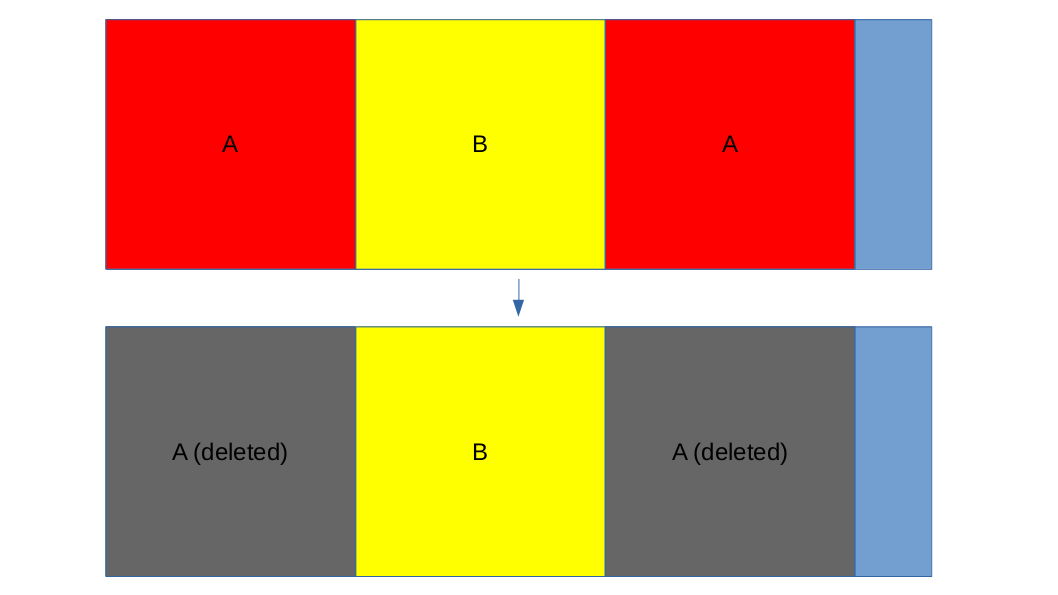
\includegraphics[width=\linewidth]{fig/case2.png}
        \caption{Test Case 2}
        \label{fig:case_2}
    \end{figure}
    \item [3]
 Deleted file fragmented around a deleted file
    \item [4i]
 Beginning of deleted file overwritten by an active file\ref{fig:case_4i}
    \item [4ii]
 Middle of deleted file overwritten by an active file
        \begin{figure}[h]
        \centering
        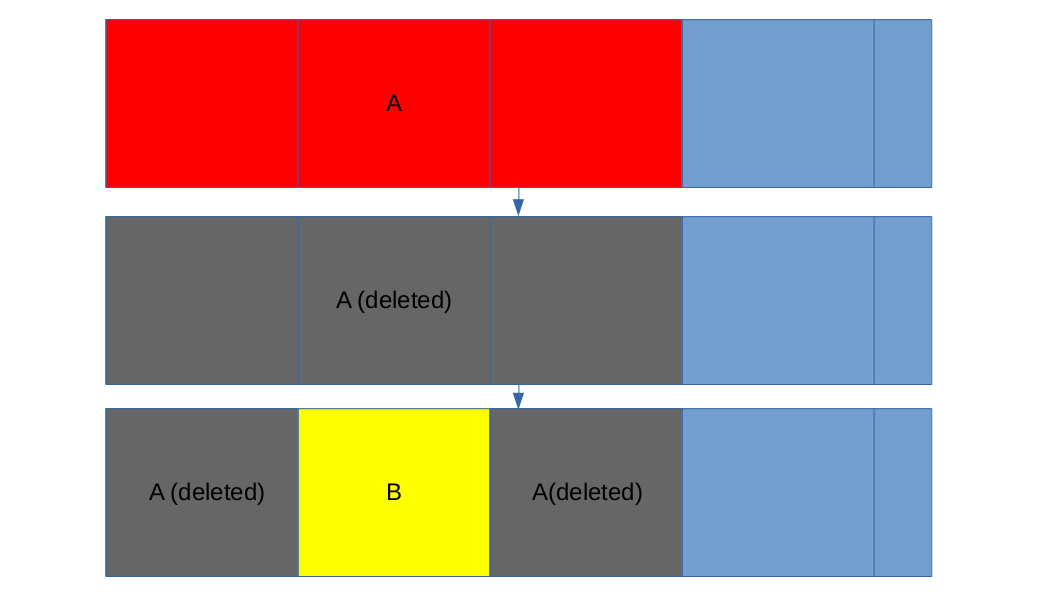
\includegraphics[width=\linewidth]{fig/case4ii.png}
        \caption{Test Case 4ii}
        \label{fig:case_4ii}
    \end{figure}
    \item [4iii]
 Deleted file partially overwritten by an active file which doesn't end on a sector boundary
    \item [4iv]
 Deleted file entirely overwritten by an active file
    \item [5i]
 Beginning of deleted file overwritten by a deleted file
    \item [5ii]
 Middle of deleted file overwritten by a deleted file
    \item [5iii]

 Deleted file partially overwritten by a deleted file which doesn't end on a sector boundary
    \item [5iv]
 Deleted file entirely overwritten by a deleted file
    \item [6]
 Deleted file fragmented around an active file, with the second fragment overwritten by an active file\ref{fig:case_6}
    \begin{figure}[h]
        \centering
        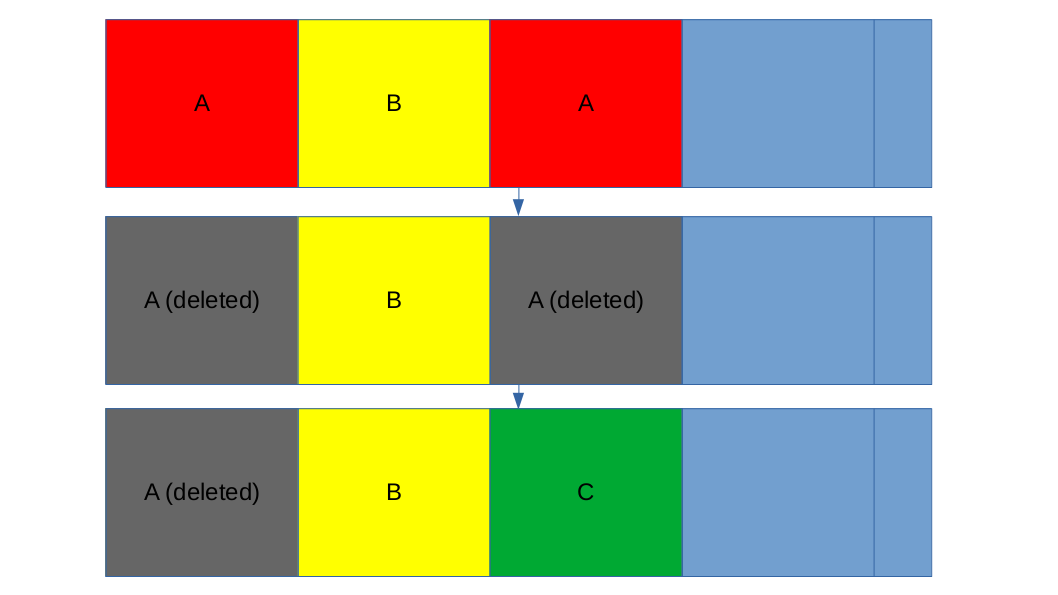
\includegraphics[width=\linewidth]{fig/case6.png}
        \caption{Test Case 6}
        \label{fig:case_6}
    \end{figure}
    \item [7]
 Deleted file fragmented around an active file, with the second fragment overwritten by a deleted file
    \item [8]
 Deleted file fragmented from the end of the filesystem to the beginning
    \item [9]
 Deleted file fragmented from the end of the filesystem to after an active file
    \item [10]
 Deleted file fragmented from the end of the filesystem to after a deleted file
\end{itemize}

Because NTFS keeps track of the locations of all parts of a file even after deletion, fragmentation is not particularly interesting. Cases 8, 9, and 10 would be redundant with case 2, so we have excluded them for NTFS. Due to how NTFS allocates space for files, cases 4ii and 5ii cannot occur as a result of normal file operations, so they have also been excluded. No cases are excluded for FAT tests.

\subsection{Creating Test Images}
% Step by step process
All test filesystems were created in partitions on a 32 GB flash drive. For each test case, the first step is to entirely write over the partition with zeros. This ensures all cases start from identical, reproduceable conditions. A new filesystem is written to the partition, then new files are written to the filesystem and deleted. The files used are simple text files containing one letter repeated (e.g. ``aa1M'' is 1 MiB of the letter 'a'). Files are written to the test filesystem by simply copying them from another drive. In some cases we also append data to a file in the test filesystem. Once the test filesystem matches the intended scenario, a read-only image of the partition is created. All tests are performed on these images rather than the original drive.

% Caching problem
It is important to consider when creating test images that the low-level behavior of file operations is not always obvious. For example, when writing a file, there is no guarantee the file's data will be immediately written to the disk. The operating system may cache the operation and wait until the optimal time to perform the write, in order to maximize system performance. We observed this early on, as writing a file and subsequently deleting it would always result in the file's metadata being written, but often left no evidence of the file's data having ever existed. This behavior is obviously undesireable because it leaves nothing meaningful to be recovered. We resolved this by calling the ``sync'' system call, which causes any such cached data to be immediately written to the disk, in between file writes and deletions. Unmounting the filesystem has a similar effect.

% Learning and using the allocation algorithms
Another type of low-level behavior relevant to the image creation process is the allocation algorithm. The operating system must have some kind of algorithm to decide where in the data area new files should be written. Common allocation algorithms include ``first available,'' ``next available,'' and ``best fit.'' %TODO cite
Learning and understanding whatever algorithm the OS uses is very helpful for forcing a specific arrangement of files. We observed that when writing to a FAT filesystem, Linux uses a ``next available'' algorithm. After the filesystem is mounted, the first write will start at the first free space in the data area. The next file will be written starting from the first free space after the previous file.
Meanwhile, when writing to an NTFS filesystem, Windows 10 appears to use a ``best fit'' algorithm. In this case, Windows tries to find the smallest space in which the file can fit without being fragmented, and write it there.

% Directory entries problem

\subsection{Recovering Files}

When testing Autopsy, we performed a standard recovery with all ingest modules disabled.
For Recuva we perfomed a standard recovery using the free version with no settings altered.
\comment{what settings did we use for FTK?}
For TestDisk we used the ``file undelete'' feature under ``Advanced Filesystem Utils.''
For Magnet Axiom we performed a ``full scan'' using the full version of the software. Magnet Axiom was tested on a separate set of filesystem images; the original images contained text files with no file extension, which Magnet Axiom did not identify. We remade the images, adding the ``.txt'' extension to all files, and tested Magnet Axiom with the new images.

\subsection{Results}

After testing each tool, we analyzed the recovered object(s) from each test case. If the recovered file is identical to the original, obviously all standards have been met. However, this only ever occurred for FAT cases 1 and 2, and NTFS cases 1-3. In all other cases, the tool is judged on each core feature individually. These judgements are summarized in the figure.\ref{fig:results}

\begin{figure}[h!]
    \centering

    \begin{subfigure}{0.3\linewidth}
        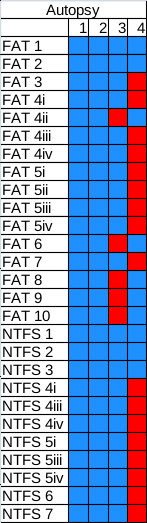
\includegraphics[width=\linewidth]{fig/autopsy_results.png}
        \subcaption{Autopsy}
    \end{subfigure}
    ~
    \begin{subfigure}{0.3\linewidth}
        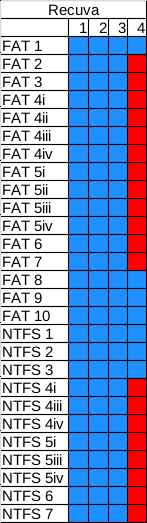
\includegraphics[width=\linewidth]{fig/recuva_results.png}
        \subcaption{Recuva}
    \end{subfigure}
    ~
    \begin{subfigure}{0.3\linewidth}
        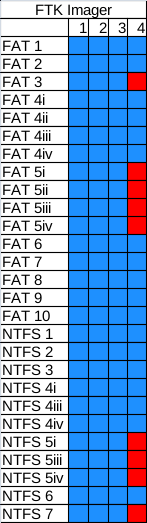
\includegraphics[width=\linewidth]{fig/ftk_results.png}
        \subcaption{FTK}
    \end{subfigure}
    
    
    \begin{subfigure}{0.3\linewidth}
        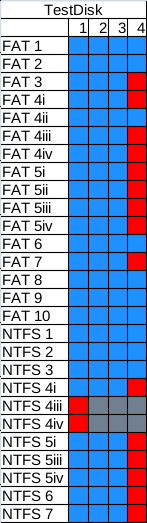
\includegraphics[width=\linewidth]{fig/testdisk_results.png}
        \subcaption{TestDisk}
    \end{subfigure}
    ~
    \begin{subfigure}{0.3\linewidth}
        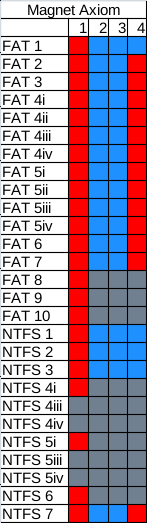
\includegraphics[width=\linewidth]{fig/axiom_results.png}
        \subcaption{Magnet Axiom}
    \end{subfigure}
        
    \caption{Test results organized by tool. Rows represent test cases while columns represent NIST core features. Blue is passing, red is failing, grey is not tested.}
    \label{fig:results}
\end{figure}

For cases in which a tool does not fulfull core feature 1, in other works, it cannot find a deleted file, we make no judgement about the remaining core features. An exception is made for Magnet Axiom, which we found does not identify certain files (text files without an extension), but can in most cases identify them when they are renamed. We consider Magnet Axiom failing to fulfill core feature 1 for all cases, and make our judgements about the other core features based on a separate set of images with renamed files. Results for NTFS cases 4iii, 4iv, 5iii, and 5iv have been excluded due to errors in the alternate test images for those cases.

In cases of fragmentation in FAT filesystems, we found each tool generally approaches recovery in one of two ways. Recuva and Magnet Axiom start from the beginning of the file and recover the full length of the file even if an active file exists in that space. Autopsy, FTK, and TestDisk will start from the beginning of the file and recover the full length, but skip over any active files they encounter. This can be seen in the results\ref{fig:results} for FAT case 2\ref{fig:case_2}. Autopsy, FTK, and TestDisk recover all of file A, while Recuva and Magnet Axiom's recovered images erroneously contain data from file B, causing them to fail core feature 4. When the space in between fragments is unallocated, all tools recover the file as though it was contiguous, pulling some erroneous data and failing core feature 4. When the fragmentation occurs at the end of the filesystem, Recuva, FTK, and TestDisk recover only the first fragment, while Autopsy returns a short file of null data, and Magnet Axiom does not identify a deleted file at all. Cases with fragmentation are trivial for NTFS filesystems as more metadata is available. Unsurprisingly, no tools had problems with fragmentation cases for NTFS.

In cases where a file has been overwritten by an active file, we found most tools recover the deleted file as though it is not overwritten, failing core feature 4. The exceptions are FTK Imager, which recovers the file up to the point where it has been overwritten, and Autopsy, which generally recovers only the first cluster of an overwritten file in FAT, and behaves like the other tools for NTFS. TestDisk also exhibits the same behavior as FTK for FAT case 4ii only. When the overwriting file has also been deleted, all tools recover the first file as though it is not overwritten.

A few results stand out as unusual. For FAT cases 4ii, 6, 8, 9, and 10, Autopsy returns a 1.5 KiB file of null data. 1.5 KiB is equivalent to 3 sectors; a FAT cluster in our cases is equivalent to 4 sectors or 2 KiB.
TestDisk fails to find a file for NTFS cases 4iii and 4iv only. Besides Magnet Axiom, these are the only test cases in which a tool does not fulfill core feature 1.

% Explain Magnet Axiom filenames issue

\section{Discussion}

\subsection{Answering Research Questions}
\subsubsection{RQ1}
Do the popular DFR tools (as available in the market) meet the NIST CFTT standards? 
If not, which tool meets which part of the standard? 

Generally, we found that the DFR tools we tested did not meet the NIST CFTT standards.
Testdisk\cite{testdisk} failed to fulfill core feature 1 because it did not identify deleted files in two test cases.
All tools fulfilled core feature 2, as they produced a recovered object for every deleted file they identified.
Autopsy\cite{autopsy} and Magnet AXIOM\cite{axiom} failed to fulfill core feature 3 because in several test cases they did not recover data they had access to.
All tools failed to fulfill core feature 4 because in many cases they recovered data which was not part of the original file.

\subsubsection{RQ2}
What factors make the tools fail or succeed?

The most common factor causing tools to fail is when a deleted file has been overwritten.
Core feature 4 requires that a tool only recover data which was originally a part of the deleted file.
A tool's success regarding this feature is thus a measure of its restraint.
The only tool to consistently fulfill core feature 4 is FTK Imager.\cite{ftk}
When it detects that a file has been partially or completely overwritten by another file, it omits the deleted sections (and everything after them in FAT).
However, in cases when the overwriting file has also been deleted, even FTK fails to fulfill this core feature.
It is worth noting that Autopsy does appear to react to overwritten files; for some cases of overwriting in FAT, it returns only a single cluster, presumably the starting cluster of the deleted file.
However, since that cluster has been overwritten, Autopsy still fails to fulfill core feature 4 in those cases.

Another factor that causes multiple failures is simulated in FAT cases 8, 9, and 10.
In FAT, a file can be written starting close to the end of the file system, without enough space to fit contiguously.
In such cases, the file must be fragmented, and since it is already at the end of the file system, the second fragment will appear closer to the beginning of the file system (this is illustrated in Figure \ref{fig:case_8}).
This scenario could realistically occcur when the file system is almost full.
In these cases, no tool is able to recover the second fragment of the deleted file; however, because FAT fragmentation is unpredictable, we only require them to recover the first fragment.
Interestingly, Autopsy and Magnet AXIOM fail to recover anything at all, with Autopsy returning a short file of null data, and Magnet AXIOM returning an empty file after displaying an error message.

\subsubsection{RQ3}
Are the free DFR tools more effective compared to the enterprise-level (proprietary) tools?

As can be observed in Figure \ref{table:results_table}, no type of tool clearly outperforms the others.
FTK Imager, a proprietary enterprise-level tool, passes the most test cases by a large margin.
However, the other enterprise-level tool, Magnet AXIOM, passes the least test cases.
Given the available data, we cannot reach a definite conclusion for RQ3.

\begin{table}[h!]
    \caption{DFR tools sorted by type. ``Passes'' refers to the number of test cases in which a tool fulfills all 4 core features.}
    \label{table:results_table}
    \begin{tabular}{| c | c | c |}
    \hline
    \textbf{DFR Tool} &  \textbf{Type} &  \textbf{Passes} \\ \hline
    Autopsy & free open source & 5 \\ \hline
    TestDisk & free open source & 10 \\ \hline
    Recuva & proprietary freemium & 7 \\ \hline
    FTK Imager & proprietary enterprise & 18 \\ \hline
    Magnet AXIOM & proprietary enterprise & 4 \\ \hline
    \end{tabular}
\end{table}    

\subsection{Ambiguity in Standards}
While determining how to interpret the NIST standards, we encountered ambiguities in their current wording.

\subsubsection{Core Feature 3 and FAT Fragmentation}
Core feature 3's requirement that a tool recover ``all non-allocated data blocks identified in a residual metadata entry''\cite{meta:dfr:standards} is not well-defined when considering a FAT file system. 
In FAT, the only relevant metadata left over after file deletion is the address of the first cluster of file data, and the file's length. 
If the deleted file is fragmented at any point, no evidence remains in the metadata. 
Therefore, interpreting the wording very closely, a tool is only required to recover the first cluster of a file's data. 
As this would not be particularly useful, it is unlikely that this was the intended meaning. 
For these tests we interpret core feature 3 as requiring the first contiguous segment of unallocated clusters starting from the first cluster originally allocated to the deleted file. 
In other words, if the file is fragmented, the tool must recover at least the first fragment. 
If a file is partially overwritten, the tool must recover at least the clusters before the overwritten part.
In essense, the tool is only required to recover data for which it does not have to guess what file the data belongs to.
However, it should be emphasized this is an assumption and the intent of the standard in this case needs clarification.

\subsubsection{Contradictory Core Features}
When designing test cases, we found situations in which core features 3 and 4 are entirely incompatible. 
Core feature 3 specifies ``all non-allocated data blocks identified in a residual metadata entry,''\cite{meta:dfr:standards} but that can sometimes still include data from other files. 
One such situation is when a deleted file is overwritten, and then the overwriting file is also deleted, such as in case 5i (as seen in Figure \ref{fig:case_5i}).

\begin{figure}[h]
    \centering
    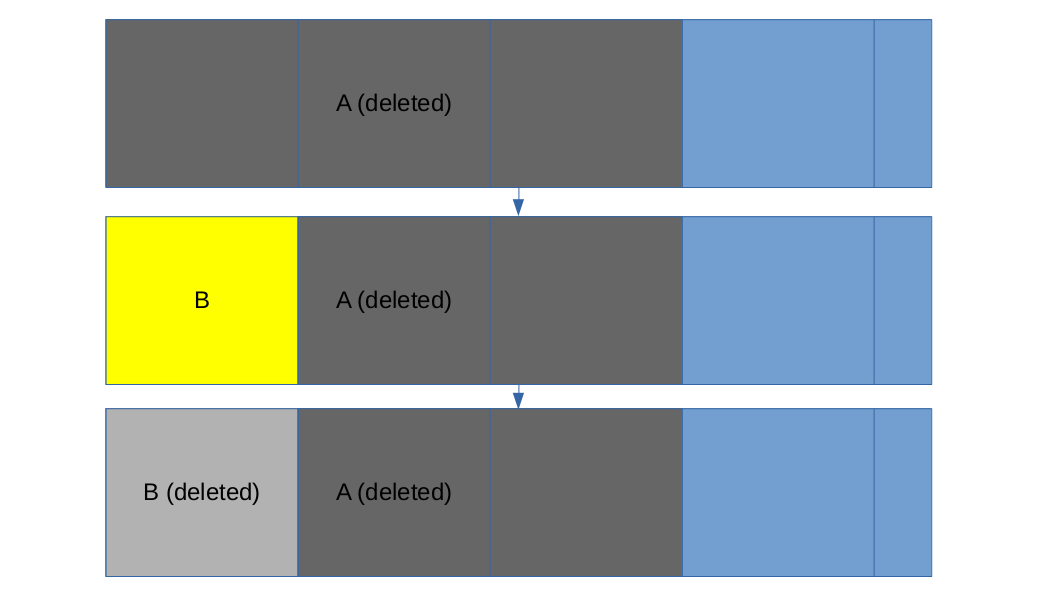
\includegraphics[width=\linewidth]{fig/case5i.png}
    \caption{Test Case 5i}
    \label{fig:case_5i}
\end{figure}

Assuming the file system is NTFS (to avoid the afforementioned ambiguity with core feature 3 and FAT), the residual metadata entry for File A (in this case its Master File Table entry) should list every cluster File A once occupied. 
All of those clusters are unallocated, so to fulfill core feature 3, the tool must recover them. 
However, some of those clusters have been overwritten by File B. Core feature 4 requires that a tool only recover ``data blocks from the Deleted Block Pool,''\cite{meta:dfr:standards} and defines the Deleted Block Pool as all blocks which ``have not been reallocated or reused.''\cite{meta:dfr:standards}
Core feature 3 would require tools to recover the clusters reused by File B, while core feature 4 would forbid this. 
It could be argued that the tool should use File B's metadata to recognize that File B overwrote File A, but this is not always realistic. 
While the file system stores information such as creation and modification times, this is not ``essential metadata,'' meaning it is not involved in the operation of the file system, so operating systems may implement it inconsistently, or not at all.\cite{carrier:filesystems}
Since the time information cannot be counted on to be reliable, there is no way to know for sure which file overwrote which. 
It is also possible for File B's metadata entry to be overwritten at some point before File A's, in which event there is no way for the tool to know File B even existed.

The standards document acknowledges that the ``potential for corruption [is] inherent with data that is no longer maintained by a file system,''\cite{meta:dfr:standards} and that the recovered object ``may not completely match the original FS-Object.''\cite{meta:dfr:standards}
We propose the standards themselves should be revised to better account for such situations.
This would most likely mean adding an exception to either the third or fourth core feature, for cases in which data blocks are overwritten and subsequently deallocated.

\subsection{Future Work}
The NIST CFTT standard includes several optional features; these features could be explored using a similar methodology.
We only created test images for the FAT and NTFS filesystems; our process could be expanded to other common filesystems such as ext4 and HFS.
NIST CFTT has a separate set of standards for file carving DFR tools; future work could involve creating test cases for file carving tools.

\vspace{-.1in}
\section{Conclusion}
\label{sec:conclusion}
\vspace{-.02in}

% We present a comprehensive analysis of the current landscape of Android malware.
% To help the research community better understand malware behavior
% and design new anti-virus solutions,
We created a large volume of well-labeled and well-studied
Android malware dataset containing \samsize samples, categorized in \versize
varieties among \fsize families ranging from 2010 to 2016.
For each variety of this dataset we 
conduct a comprehensive study to profile their behaviors and evolution trends.
We document in details the process of creating this dataset to enable other
researchers to replicate the process.
We observe that Android malware are evolving towards monetization, and becoming
sophisticated and persistent.
The extensive usage of anti-analysis techniques in the malware samples
shows the urgent need for advanced de-obfuscation and dynamic analysis methods.
We will make the dataset available to research community.

%%% Local Variables: 
%%% mode: latex
%%% TeX-master: "paper"
%%% End: 


\ack A. Meyer's work has been partially supported by a grant from BGSU's Center for Undergraduate Research and Scholarship 
(CURS) in summer of 2019. S. Roy's work has been partially supported by a NIST grant (grant number: 70NANB17H321; Year 2017-19) that he has been awarded with as a Co-PI. 
Quinton Currier at BGSU assisted with the testing process.

\bibliographystyle{icstnum}
\bibliography{mybib}

\end{document}
